\documentclass[11pt]{article}

\usepackage{graphicx}
\usepackage{caption}
\usepackage{amsfonts}
\usepackage{xcolor}
\usepackage{subfig}
\usepackage{subfloat}
\usepackage{hyperref}
\usepackage{eurosym}

\graphicspath{{IMG/}}
	
\begin{document}
    \raggedbottom
    \sloppy \lefthyphenmin=1000
    \setlength{\parskip}{3ex}

\title{NEW Infrastructures and Risk assessment overview}

\author{J. Toledo}


\maketitle

\section{Scope and outlook}

The present document provides an overview of the hazards in the NEW detector operation.
The basic design and operation parameters for NEW are also presented.

\begin{figure}[ht!]
    \bigskip
    \begin{center}\leavevmode
        \rotatebox{0}{
        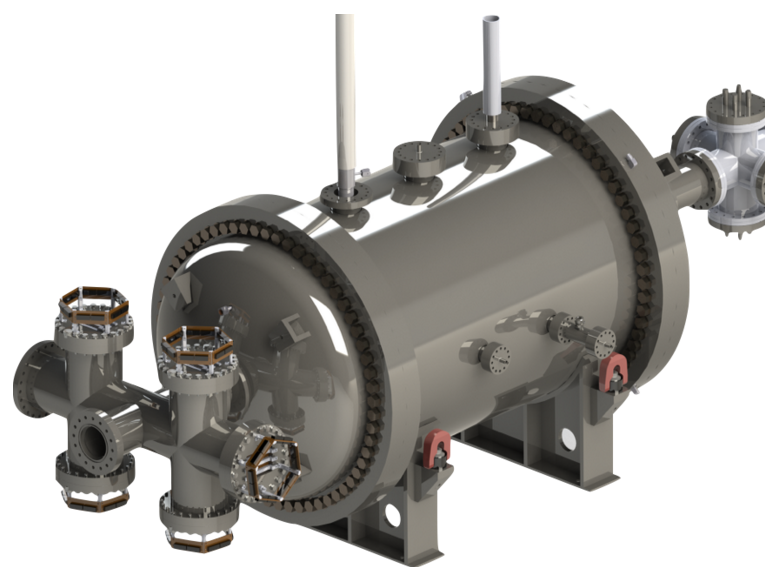
\includegraphics[width=\textwidth, ]{F0.png}}
        \caption{\textit{The NEW vessel with stands, high-voltage feedthroughs (top), energy plane feedthrough and cross (right) and 
        tracking plane feedthrough with "spaceship"� multi-port pipe (left)}}
        \label{fig:F0:F0}
    \end{center}
\end{figure}


\subsection{Risk assessment purpose}
Throughout the risk assessment review, the NEXT Collaboration requests permission to LSC to operate the NEW detector with Ar and depleted Xe, 
with pressure in the vessel in the range 5-10 bar (matching the compressor's input range). After a period of operation, the Collaboration will 
request permission to operate with enriched Xe, which will imply a new risk assessment process.

Under such circumstances, the loss of gas (Ar or depleted Xe) is not considered a hazard in the current stage, though we have designed the Gas System 
to address such potential events (via an emergency recovery tank and a cry-recovery bottle). The term "hazards"�will be limited to situations that could 
result in damage to personnel or LSC infrastructures.
 
 \subsection{General LSC safety rules}
LSC establishes access control rules, general safety rules and emergency rules (see http://www.lsc-canfranc.es/en/safety.html). 
NEXT personnel is trained in these rules, including special training courses for those individuals distinguished as team responsible persons.

LSC general safety rules require that personnel underground wear safety shoes and reflective vest. Access to the pool requires also the use of a helmet. 
The two-person rule must be followed (working underground requires the presence of a second person who might help and intervene in case of accident or emergency).
				
LSC safety rules for experiments are described in the document "Safety Guide for Experiments v0 Rev4". 
This document is available online http://www.lsc-canfranc.es/Docs/Safety/LSC\_Experiments\_SG.pdf.


\section{Hazards associated to NEXT infrastructures}
NEXT occupies the far end of the Hall A. A supporting structure with tramex floor delimits the 11x11 m2 NEXT experimental area and working platform. 
Under the platform, and covering most of Hall A extension, a large pool exists to protect personnel from gas and liquid dumps.

\begin{figure}[ht!]
    \bigskip
    \begin{center}\leavevmode
        \rotatebox{0}{
        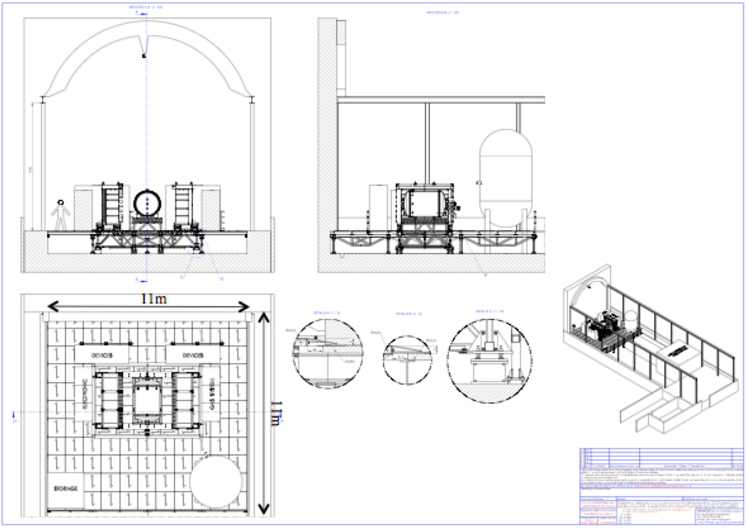
\includegraphics[width=\textwidth, ]{F1.png}}
        \caption{\textit{The NEXT experimental area in Hall A at LSC. Actual recovery tank (bottom left corner in the 11x11 m2 platform) is placed horizontally}}
        \label{fig:F1:F1}
    \end{center}
\end{figure}

\subsection{Gas venting and asphyxiation hazard}
In the case of NEW, the amount of Xe liberated in a catastrophic failure (vessel rupture, bursting disk rupture by overpressure) would be less than 1.5 m3 and it does 
not represent any asphyxiation hazard, given its small volume compared with the total volume of the experimental hall and the presence of the pool, where gas 
(Ar and Xe are heavier than air) will sink  to a thickness of less than 1 mm.

Nevertheless, the pool does not currently have any ventilation. Only a perimetral liquid sink exists. 
Air intakes are placed in Hall A in the pillars, at about 30 cm above the working platform. 
Air quality might be monitored with some periodicity in the pool by LSC, as other experiments in Hall A (like ArDM) might dump gas too.


Maintenance work under the platform does not require any safety measures other than wearing a helmet, according to LSC rules. 
This provides access to the cable trays (signal and power) and pipes that run under the tramex.

\begin{figure}[ht!]
    \bigskip
    \begin{center}\leavevmode
        \rotatebox{0}{
        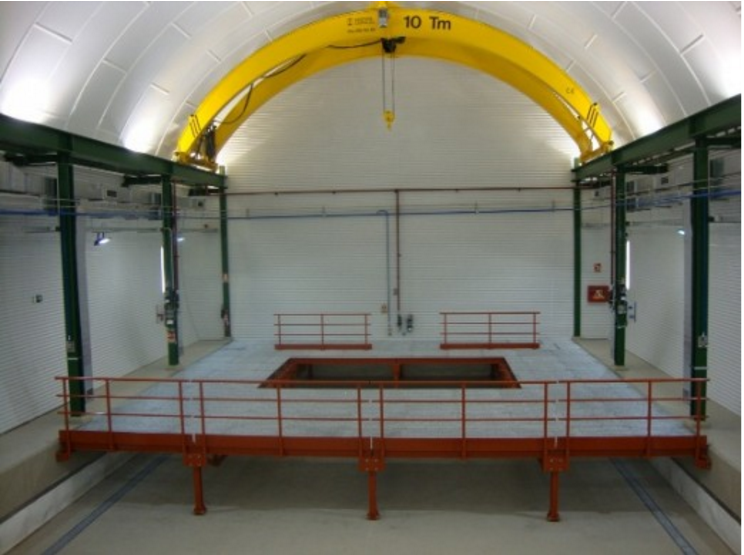
\includegraphics[width=\textwidth, ]{F2.png}}
        \caption{\textit{The NEXT working platform, empty}}
        \label{fig:F2:F2}
    \end{center}
\end{figure}

\subsection{Seismic hazard}
A seismic structure, designed according to national regulations and approved by LSC, occupies the center of the working platform. 
The NEW vessel and lead castle are mounted on top of the pedestal. 

The structure is described in detail in the companion document Seismic\_report.pdf, "NEXT-100 project: Structural Seismic Analysis",  Release 1.0 October 17, 2012.

As a result of the HAZOP analysis, we plan to add an accelerometer to detect earthquaques and bring NEW to a safe state. This additional safety measure will be implemented before end of 2016.

\begin{figure}[ht!]
    \bigskip
    \begin{center}\leavevmode
        \rotatebox{0}{
        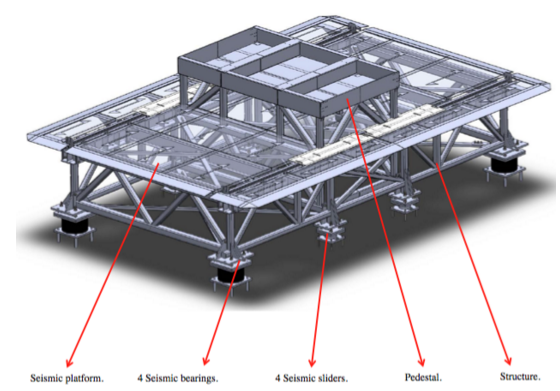
\includegraphics[width=\textwidth, ]{F3.png}}
        \caption{\textit{The seismic platform}}
        \label{fig:F3:F3}
    \end{center}
\end{figure}

\subsection{Hazards related to the lead castle}
The lead castle has two moving halves, each consisting of a steel structure supporting lead bricks in the walls and in the roof. 
A safe operation protocol for the opening and closing the the castle, approved by LSC, can be found in Process Procedure NEXT-NEW-001 
(Process Procedure: Opening and closing the NEXT experiment lead castle).

\begin{figure}[ht!]
    \bigskip
    \begin{center}\leavevmode
        \rotatebox{0}{
        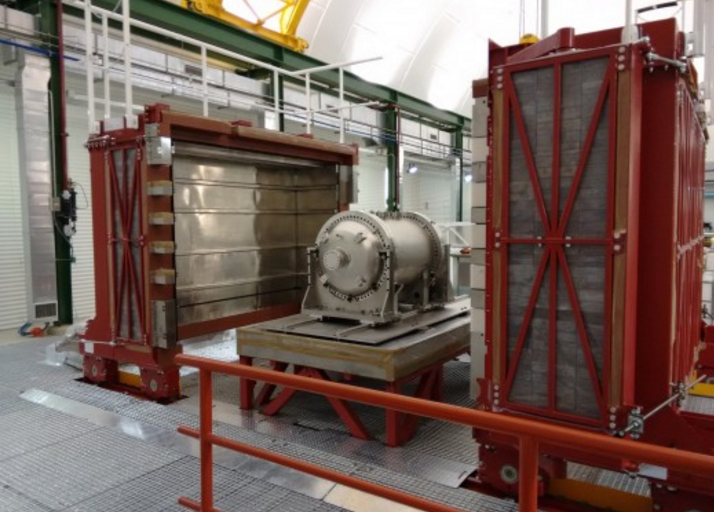
\includegraphics[width=\textwidth, ]{F4.png}}
        \caption{\textit{The lead castle in open position}}
        \label{fig:F4:F4}
    \end{center}
\end{figure}


\subsection{Hazards related to liquids}
Only two potentially hazardous liquids are used in NEXT:

\begin{itemize}
\item The chiller is filled with a solution of water and ethylene-glycol (20-30\% in volume). An estimated total volume of less than 10 liters of ethylene glycol will be used. 
As this is a combustible liquid, the stock must be stored in the red chemicals cupboard in the main corridor. 
Ethylene glycol breaks down in air in about ten days, and in water or soil in a few weeks. 
We do not expect to produce any waste of it, though any liquid spilled will be collected by the perimetral liquid sink in the pool.
\item Liquid nitrogen is used in the cryo-recovery bottle only when a cryo-recovery operation is to be carried out. 
Liquid nitrogen is stored in a room in the main corridor. A wheeled container will be filled, pulled to the NEXT experimental area, and trained personnel will fill the recovery bottle. 
LSC has a well defined safety procedure for the use and handling of liquid nitrogen in the laboratory, which we will follow 
(LSC's document "Instrucciones de operaci\'on y seguridad NITROGENO LIQUIDO.pdf".
\end{itemize}

\begin{figure}[ht!]
    \bigskip
    \begin{center}\leavevmode
        \rotatebox{0}{
        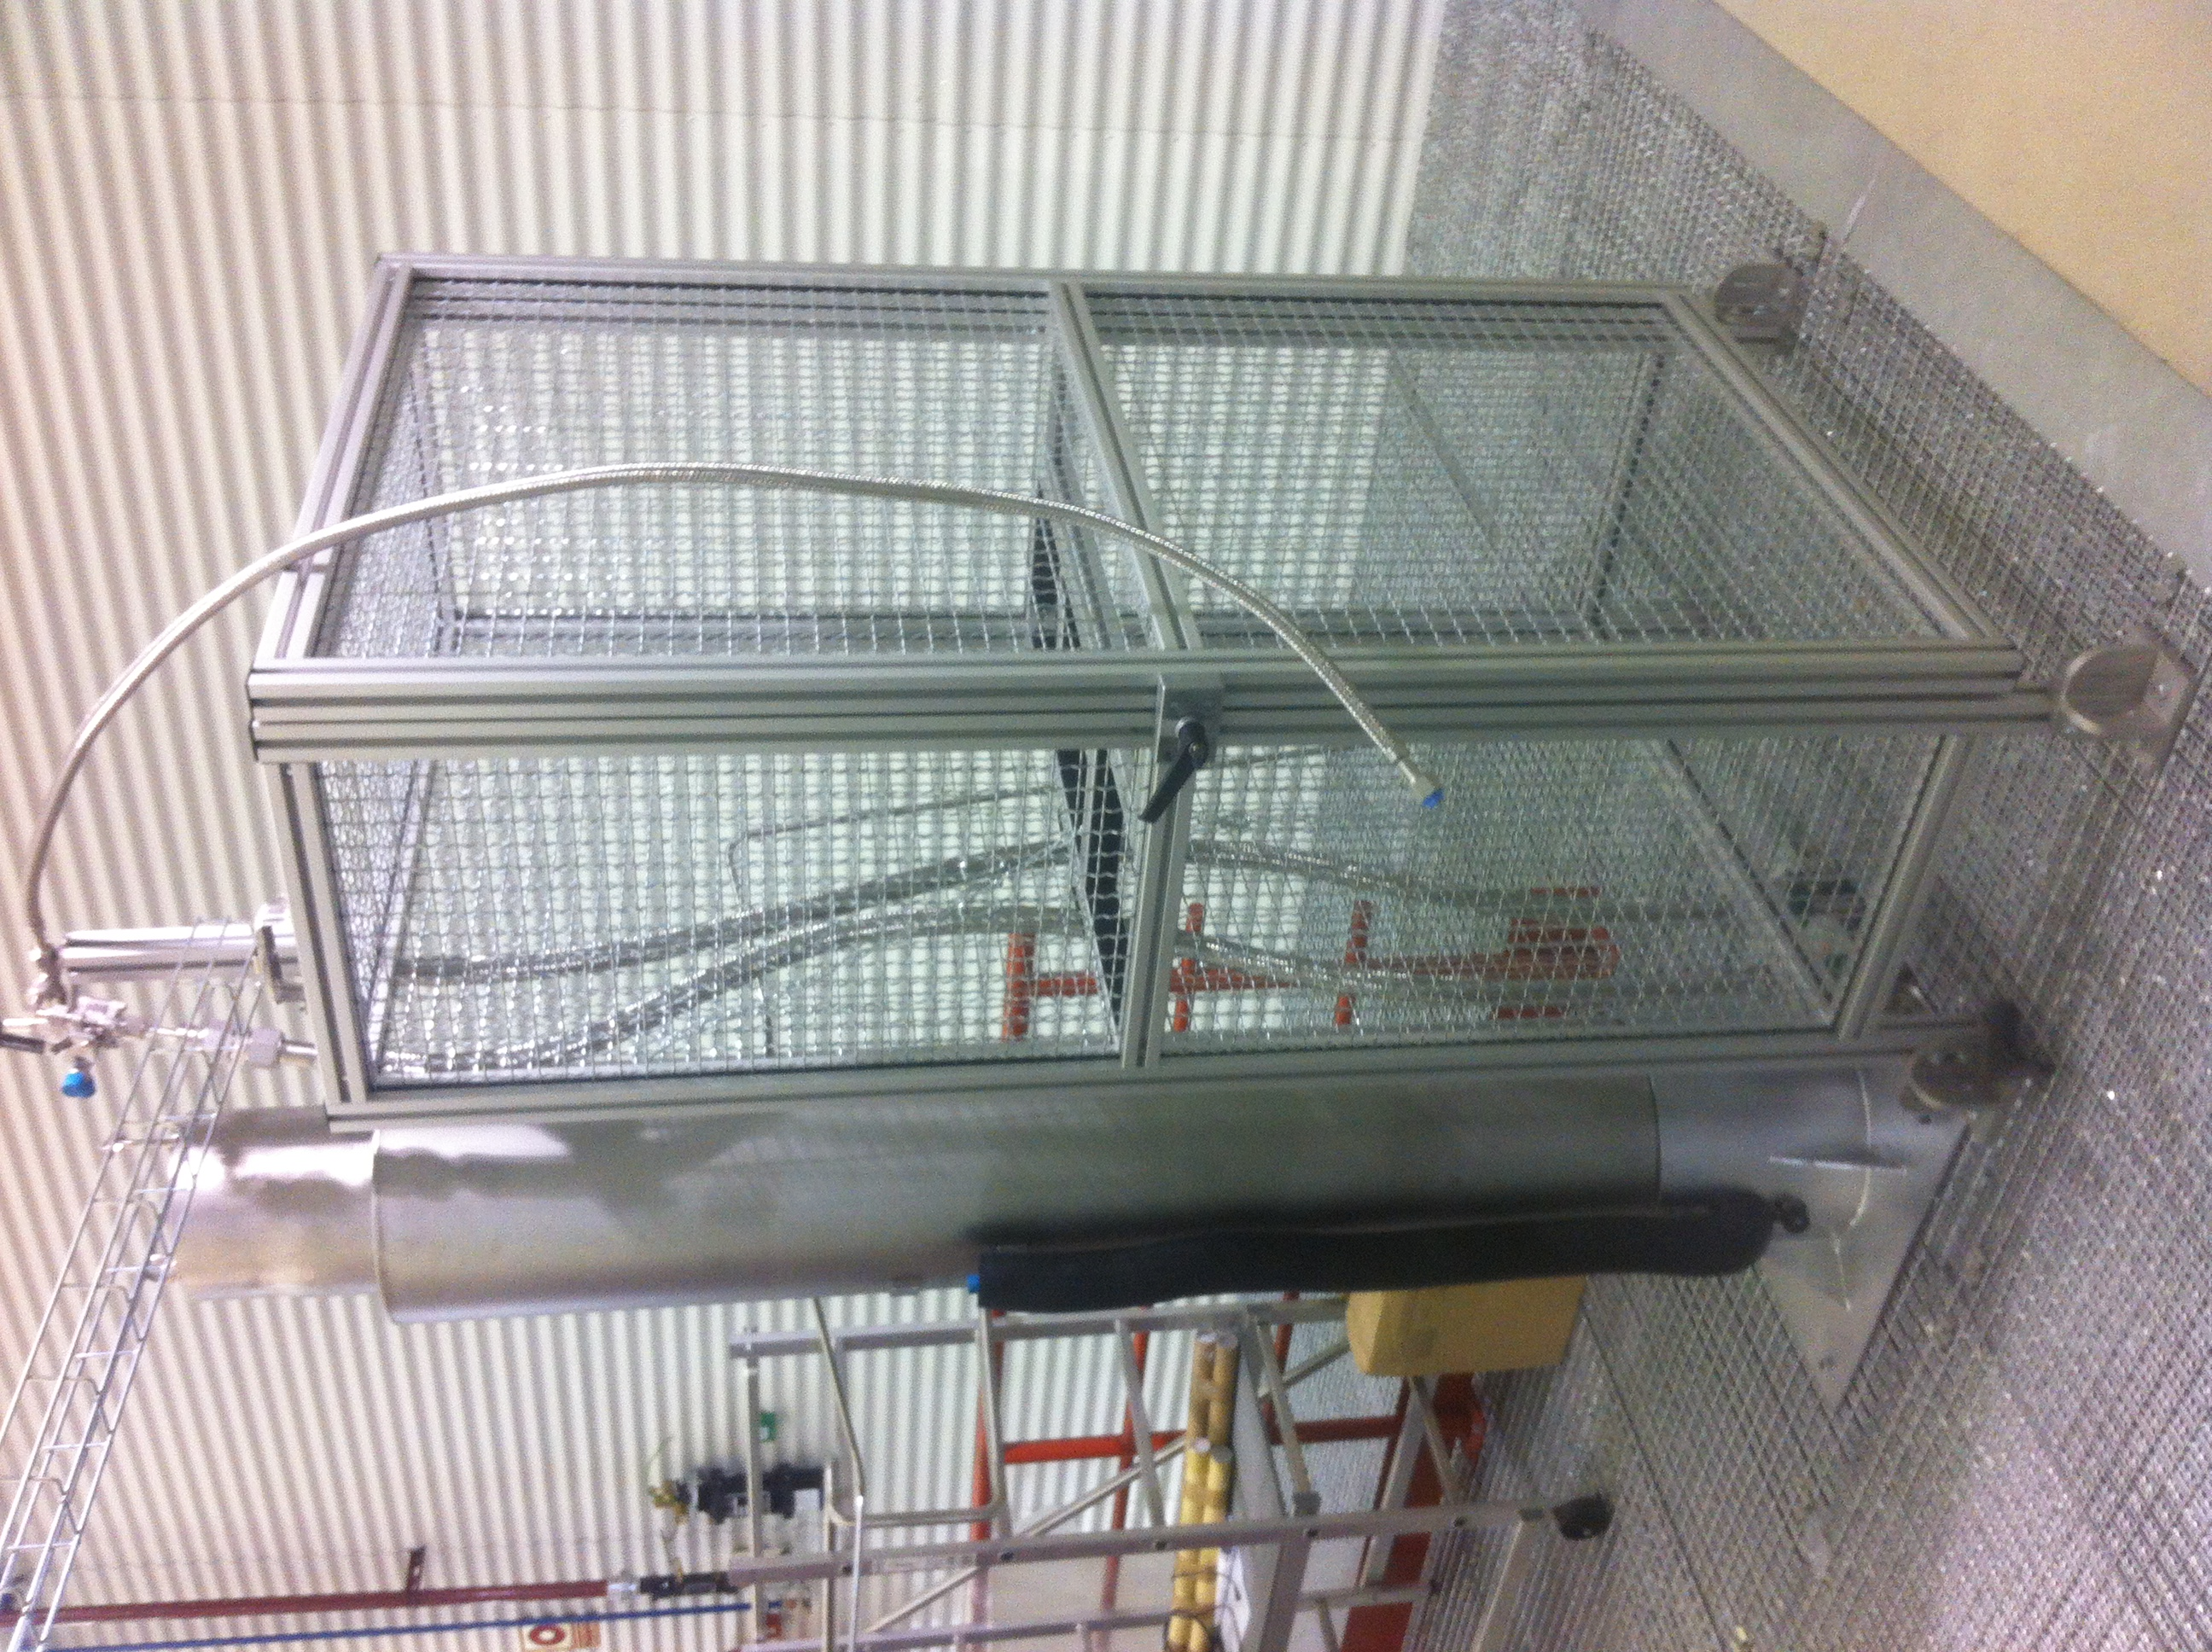
\includegraphics[width=\textwidth, ]{cryo_stand.JPG}}
        \caption{\textit{The Cryo-recovery bottle (left) and Gas bottle stand (right) on the NEXT working platform}}
        \label{fig:cryo_stand:cryo_stand}
    \end{center}
\end{figure}



\section{Hazards associated to equipment on the NEXT platform}
This section summarizes the different elements on the working platform and its hazards, especially others than those related to the Gas System and the Electronics. 

Hazards associated with the Gas System (NEW vessel, recovery talk, compressor, chiller, recirculation circuit, cryogenic recovery bottle and a number of manual and pneumatic valves) 
are described in more detail in document "Process Procedure NEXT-NEW-009: Operation methods and procedures relating to NEW Gas System"�, as well as in a number of analysis documents 
for the Gas System (FMECA analysis and report, Fault Tree Analysis, Fatigue analysis and Criticality analysis). 
A HAZOP analysis has been carried out by Insegma (www.insegma.com) in March-April 2016 (report to be released in April 2016).

\begin{figure}[ht!]
    \bigskip
    \begin{center}\leavevmode
        \rotatebox{0}{
        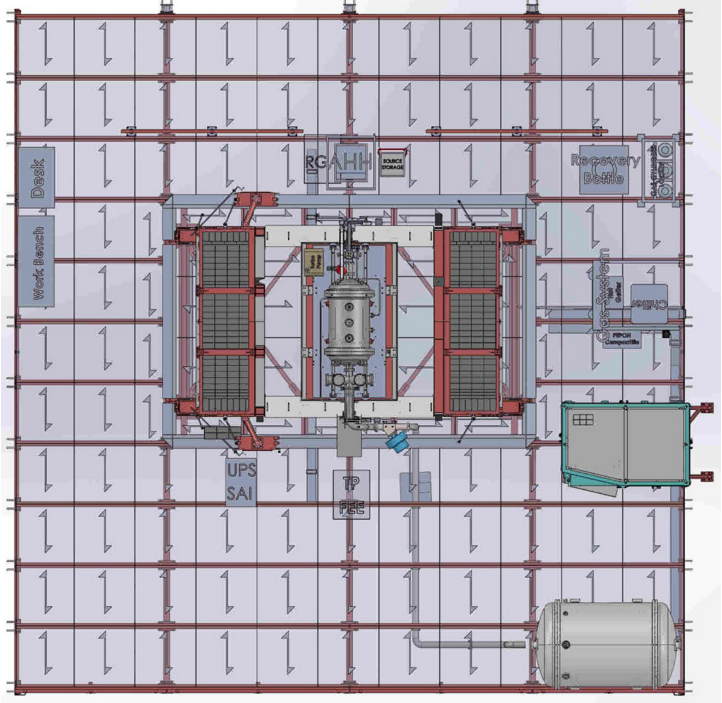
\includegraphics[width=\textwidth, ]{F6.png}}
        \caption{\textit{Layout of the NEXT working platform}}
        \label{fig:F6:F6}
    \end{center}
\end{figure}

Hazards associated with the electronics (Energy Plane rack, Tracking Plane rack, DAQ Computing rack, Very High Voltage rack, Slow Controls, and UPS units) are addressed in 
"Overview of the Risk Assessment for Electronics in the NEW detector" and more specifically in the FMECA table and report 
files FMECA\_Electronics\_NEW\_v1.xls and FMECA\_Report\_Electronics\_NEW\_v1.pdf). 

\subsection{Issues related to NEW vessel}
The center of the stage shown in figure \ref{fig:F6:F6} is occupied by the NEW vessel. It is a tank with a volume of 0.169 m3 made of 316Ti material and with CE certification at 20 bar and vacuum. 
Bursting disks and an automatic venting procedure to the recovery tank are used to safeguard against overpressure.

The vessel can be divided into three parts: (1) the central one, or active area, where the pressure will be up to 15 bar (2) the Energy Plane volume (right) which is hold at 10-6 mbar 
vacuum and (3) the Tracking Plane volume, in pressure equilibrium with the active volume.

The main issues associated with this component is a vessel rupture due to overpressure or a gas leak due to material fatigue or o-ring breach. 
The use of bursting disks and an automatic venting to the emergency recovery tank mitigate the risk of overpressure.

\begin{figure}[ht!]
    \bigskip
    \begin{center}\leavevmode
        \rotatebox{0}{
        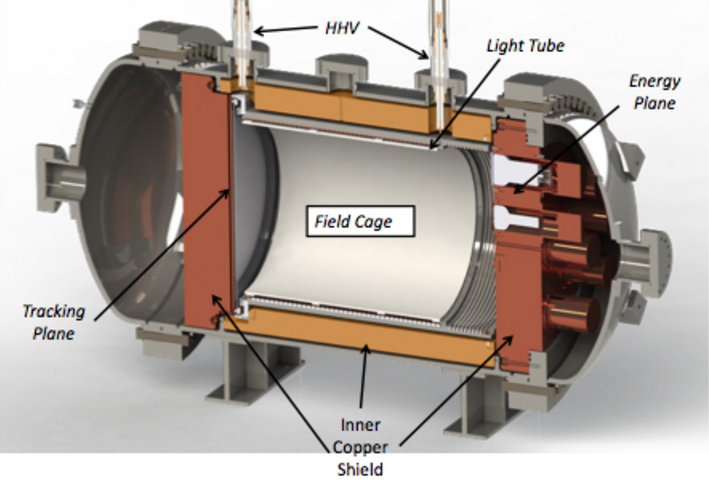
\includegraphics[width=\textwidth, ]{F7.png}}
        \caption{\textit{ A section of the NEW vessel}}
        \label{fig:F7:F7}
    \end{center}
\end{figure}

NEXT-NEW-009 details the operating procedures designed to minimize loss of gas in the case of leak in the Gas System (including the vessel). 
Nevertheless, in this stage, the NEXT Collaboration is requesting permission to operate with Ar and depleted Xe only and so this should not be considered a hazard.

In the unlikely case that a vessel rupture provokes an explosion, which is the only hazard for personnel associated with the NEW vessel, the castle acts as a shield.

\subsection{Hazards with other components in the Gas System}
The recovery tank for NEW is the NEXT-100 vessel (volume of 2,558 m3 made of 316Ti with a CE certification at 15 bar). 
It is kept at at 10-5 mbar during normal operation by the action of PUMP1 (figure \ref{fig:F8:F8}). The size of the tank ensures that after an emergency recovery situation the final 
absolute pressure is in the order of 1 bar. Thus, this component poses no hazards to the LSC installations or to personnel. Still, a bursting disk (BD1) prevents excessive 
pressure in the tank (BD1 breaks at 5 bar).

The cryo-recovery bottle has a volume of 0.060 m3. It is made of 316Ti and has CE certification at 130 bar. It is mounted on a base firmly screwed to the tramex floor. 
A bucket encloses the bottle. The bucket is filled with liquid nitrogen to reclaim the gas from the recovery tank. 
Xe is liquid at -110�C and with liquid nitrogen the temperature of the bottle will be lower than -110�C, but not enough to liquify Ar. 
During normal operation the bottle is kept at vacuum and without liquid nitrogen (only required during a cryo-recovery operation).

Hazards related with this component are (1) damage to personnel due to an accident handling of the liquid nitrogen, (2) explosion due to material fatigue or overpressure. 
The former requires to follow LSC's liquid nitrogen handling protocol. The latter is mitigated by the presence bursting disks.

The getters pose no hazards for personnel or LSC infrastructures. 
The same can be said of vacuum pumps 1, 2 and 3. The hot getter is self monitoring. It will shut down in the event of a detected fault and the gas flow will be re-directed through an 
internal by-pass line. The cold getters are passive and need to be replaced when the captured impurities reduce the gas flow (a piece of software monitoring pressure gauges PG5 and PG6 
can give a hint on when the getters are to be replaced).

\begin{figure}[ht!]
    \bigskip
    \begin{center}\leavevmode
        \rotatebox{0}{
        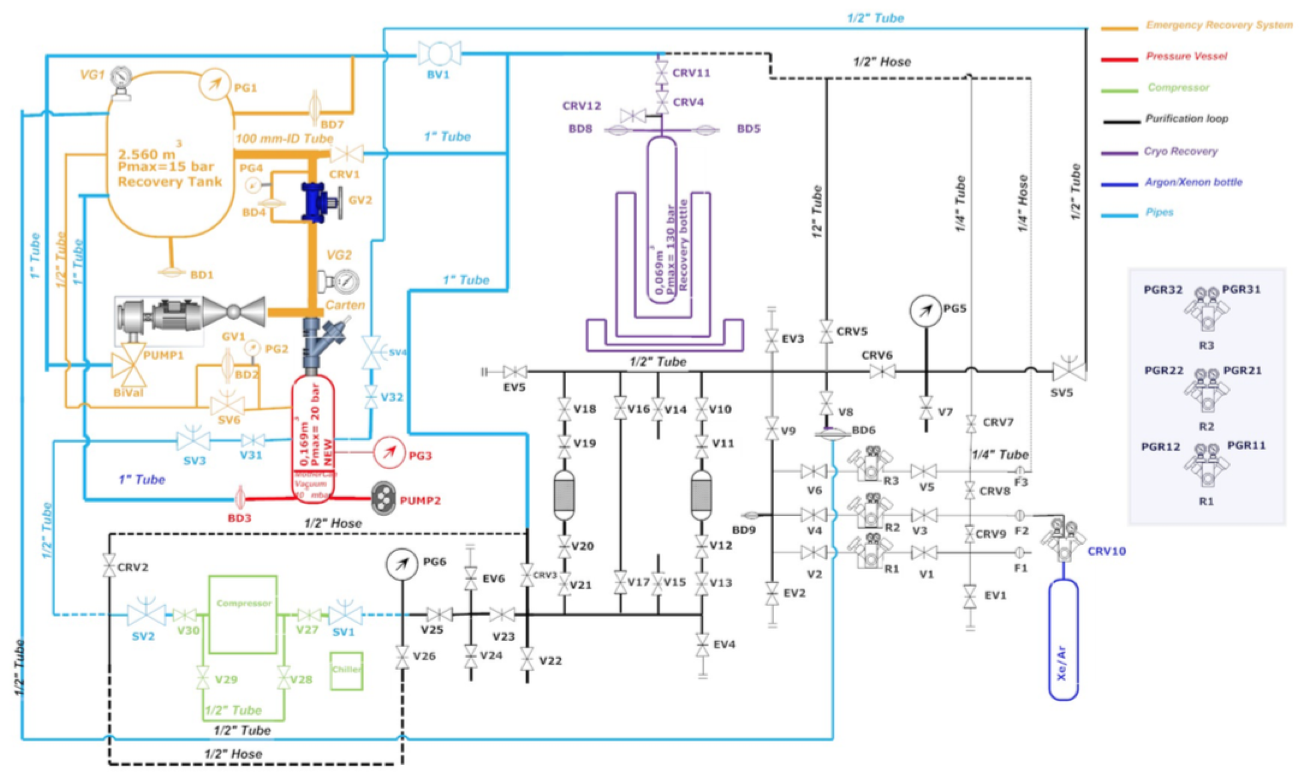
\includegraphics[width=\textwidth, ]{F8.png}}
        \caption{\textit{The NEW Gas System}}
        \label{fig:F8:F8}
    \end{center}
\end{figure}

\begin{figure}[ht!]
    \bigskip
    \begin{center}\leavevmode
        \rotatebox{0}{
        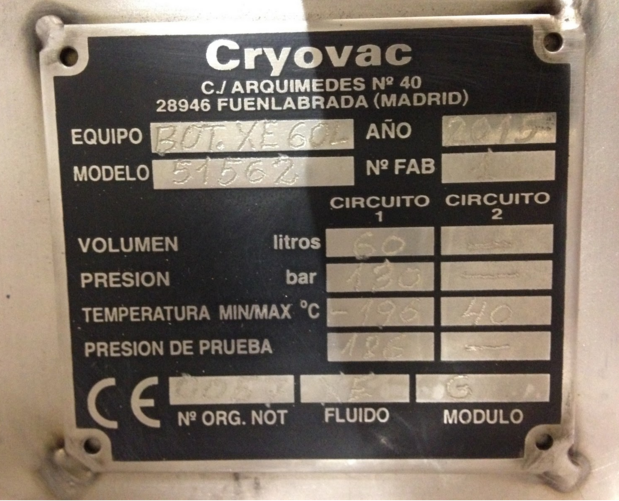
\includegraphics[width=\textwidth, ]{F9.png}}
        \caption{\textit{CE plate for the cro-recovery bottle}}
        \label{fig:F9:F9}
    \end{center}
\end{figure}

The role of the compressor is to move the gas through the purification loop. 
It is a very reliable device (figure \ref{fig:F13:F13}) having triple diaphragms to compress the gas. 
In addition, monitoring of leaks between diaphragms insures high reliability of the unit and makes the probability of gas loss highly improbable. 

The compressor can operate in two modes: (1) It will either simply move the gas through the purification circuit at a nominal pressure of 5 to 10 bar, or 
(2) it will also re-pressurize the gas in the NEW vessel to a working pressure of 15 bar. The ultimate working pressure of the compressor is 25 bar.

\begin{figure}[ht!]
    \bigskip
    \begin{center}\leavevmode
        \rotatebox{0}{
        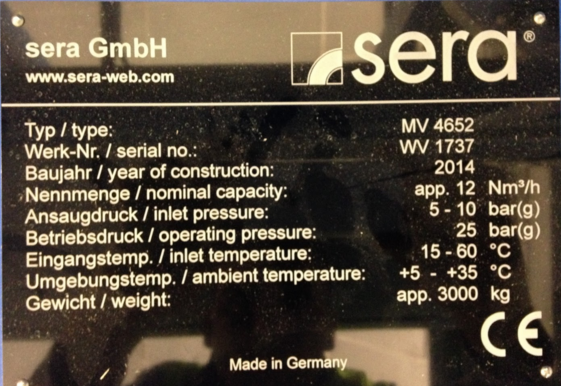
\includegraphics[width=\textwidth, ]{F10.png}}
        \caption{\textit{CE plate of the compressor}}
        \label{fig:F10:F10}
    \end{center}
\end{figure}

In case of diaphragm breach, hydraulic oil leak or other failures detected by the built-in monitoring system, the compressor will be automatically turned off and isolated from the gas system 
(by means of pneumatic valves SV1 and SV2 actuated from the cRIO chassis). 

Gas temperature needs to be monitored to avoid exceeding the range of the compressor (60�C). Coolant max. temperature in the chiller is 43�C.

The compressor needs external cooling, so a chiller unit will remove heat through a heat exchanger. A failure in the chiller will also turn off and isolate the compressor. 
These measures limit the extent of gas loss and gas overheating, being the latter the most important hazard associated with the compressor.

\begin{figure}[ht!]
    \bigskip
    \begin{center}\leavevmode
        \rotatebox{0}{
        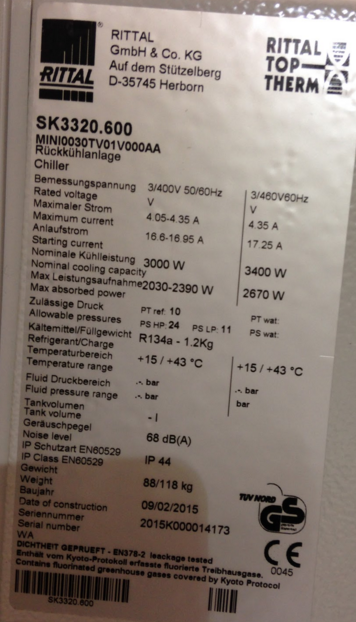
\includegraphics[width=\textwidth, ]{F11.png}}
        \caption{\textit{CE plate of the chiller}}
        \label{fig:F11:F11}
    \end{center}
\end{figure}

The regulator bottles with pressure gauges (R1, R2 and R3 in figure \ref{fig:F8:F8}) are used to fill the gas system with Ar or Xe to a desired pressure. 
Pressure gauges on both ends of each regulator, as well as in other points of the circulation loop (like PG3, PG5 and PG6), together with a well defined protocol 
(see Initial fill procedure in NEXT-NEW-009) minimize the risks of overpressure, which is the main hazard for this set of components. 

In case of overpressure, BD6 will protect the hot getter. The total amount of gas in the supply bottle and also in the system will be such that in the event of the entire bottle emptying 
into the system and being vented into the emergency recovery tank the final pressure will not exceed 3 bar.

\begin{figure}[ht!]
    \bigskip
    \begin{center}\leavevmode
        \rotatebox{0}{
        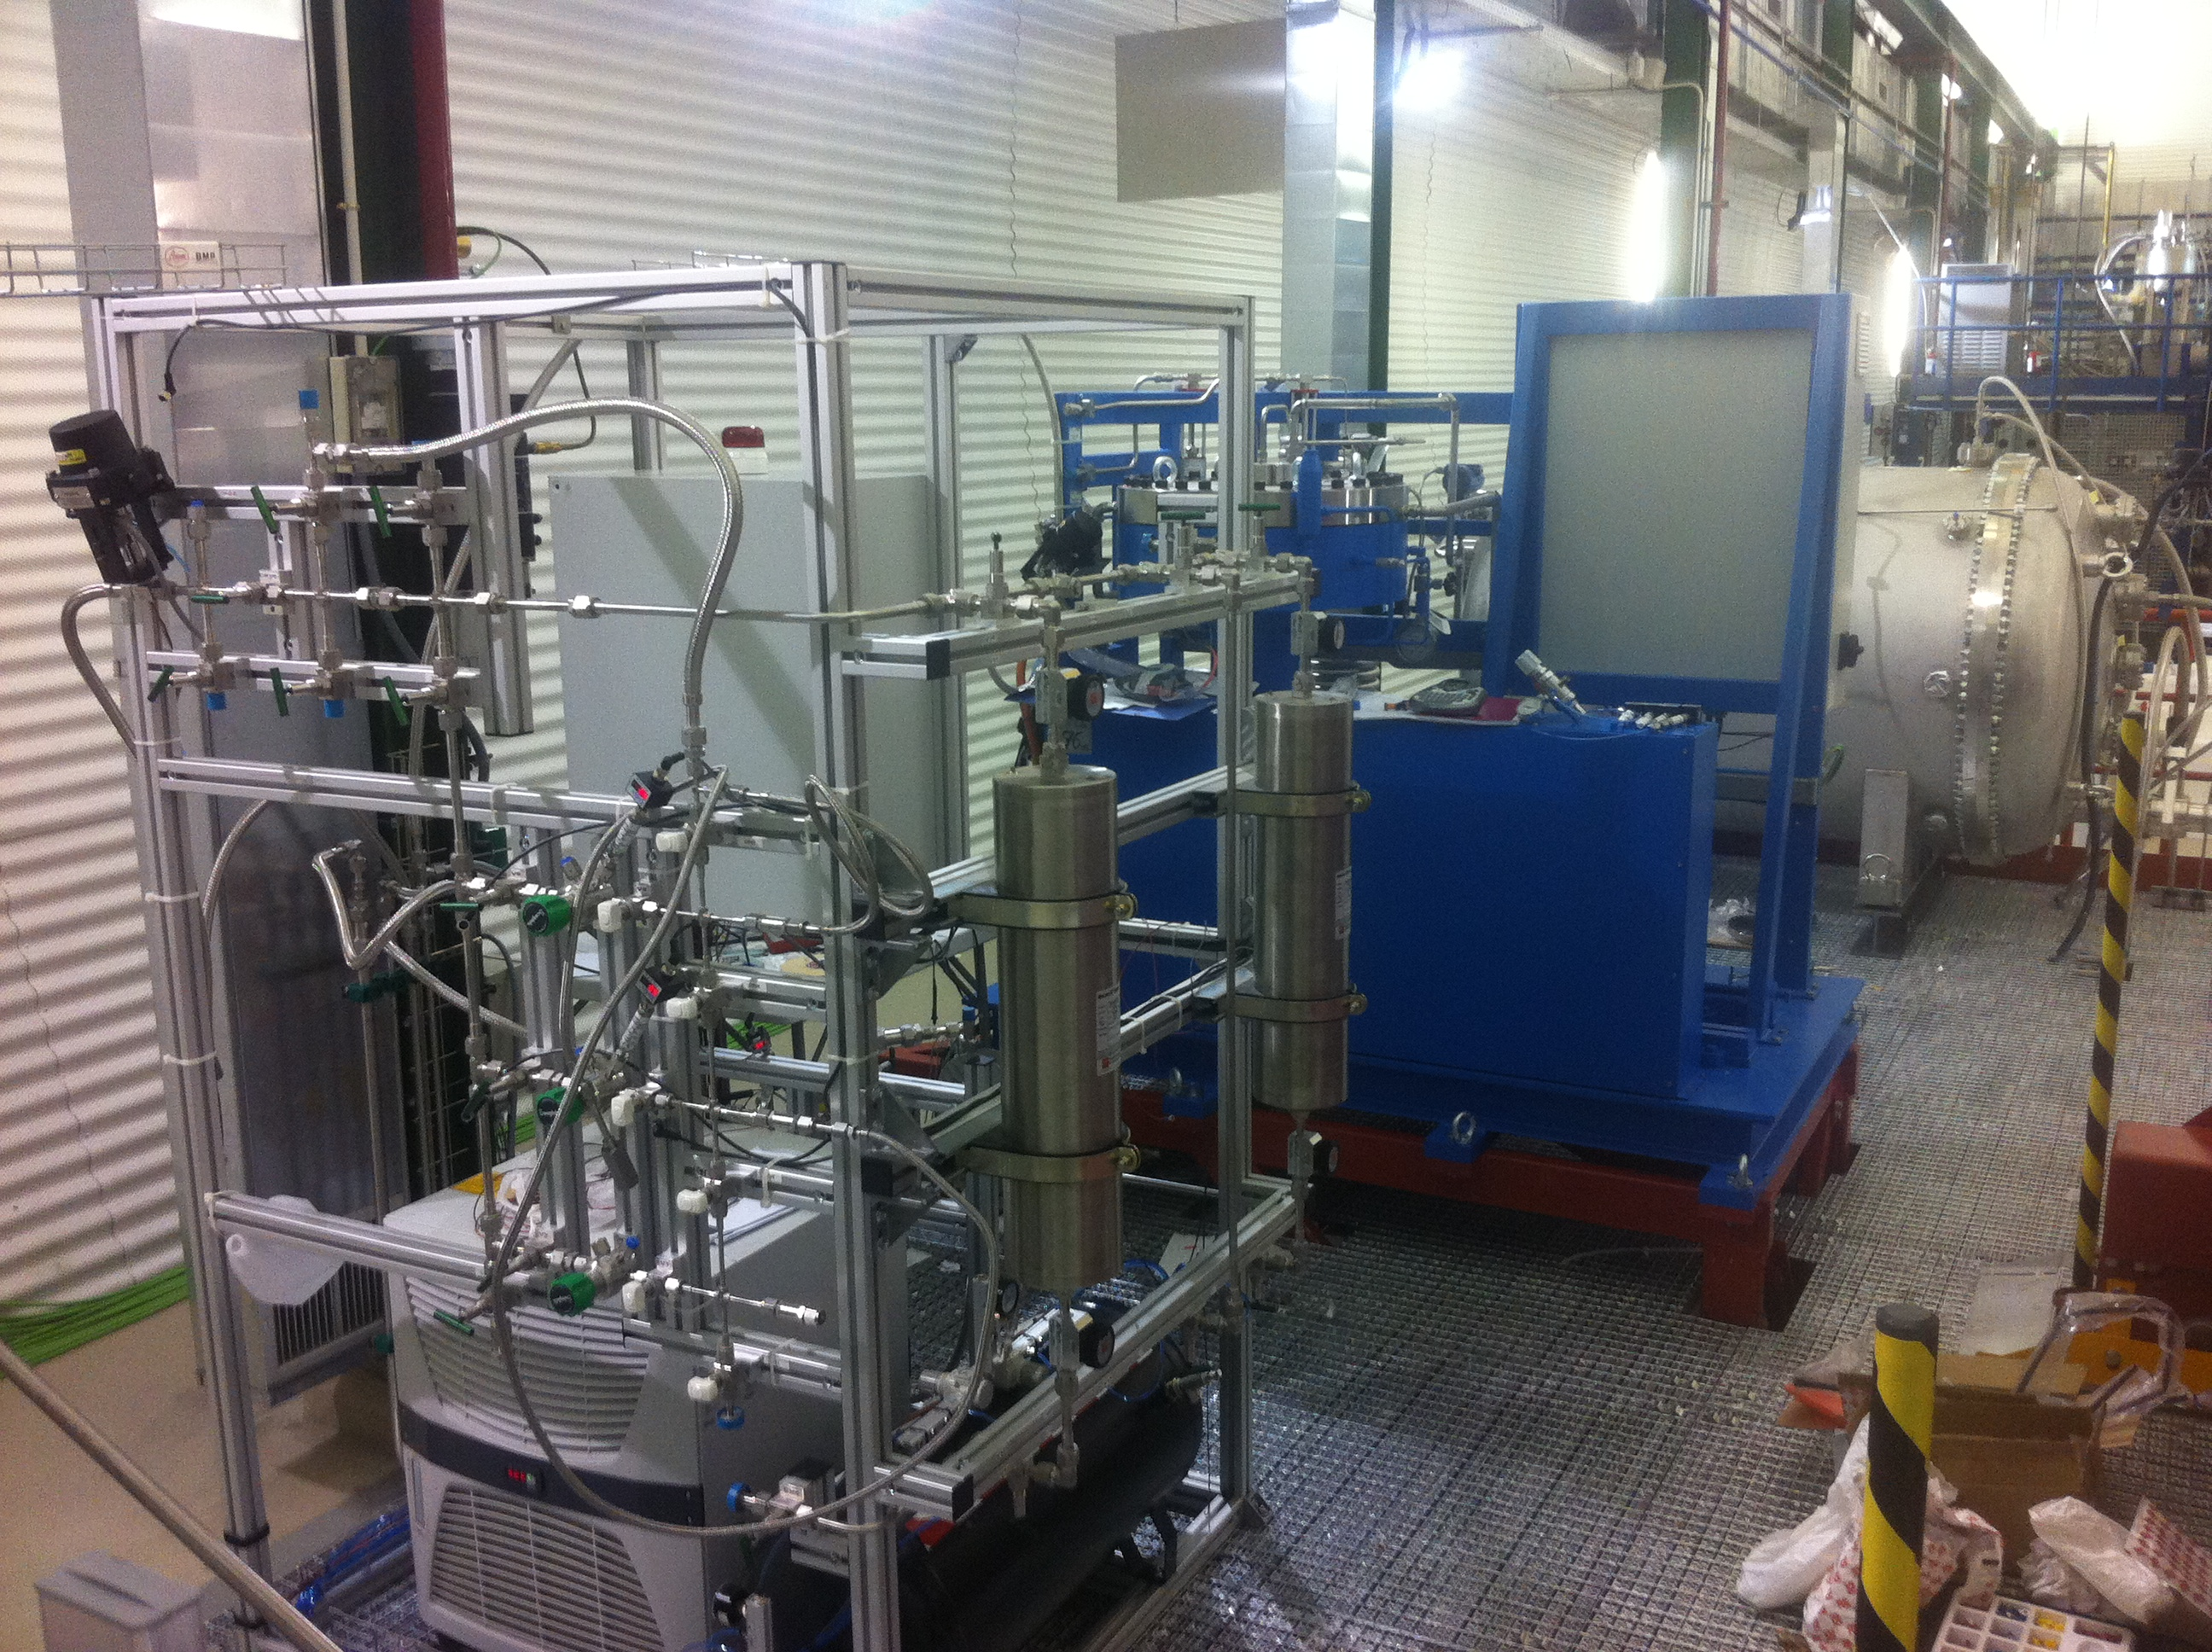
\includegraphics[width=\textwidth, ]{F12.JPG}}
        \caption{\textit{The Gas System Frame accommodates most of manual valves, the getters (only the cold getters are shown) and the regulator bottles with gauges}}
        \label{fig:F12:F12}
    \end{center}
\end{figure}

\subsection{Noise hazards}
There are two potential sources of high noise: the compressor and the (intentional) venting of the NEW vessel.

Regarding the compressor, a CE-mark product by the German company SERA, noise could be as high as 76 dB SPL. 
This level can be quite annoying (like road traffic a few meters away or a very very loud conversation).

A pedestal has been built to support a bare compressor (as shown in the picture above) and, if required, a compressor surrounded by a isolating structure. 
LSC has assumed the responsibility to build and install such structure if the noise level in Hall A turns out to be beyond acceptable levels.

Regarding the noise produced when (intentionally) venting the NEW vessel during the test phase, a protocol to carry out this operation has been approved by LSC and is described in 
Process Procedure NEXT-NEW-003, section 9B.

\begin{figure}[ht!]
    \bigskip
    \begin{center}\leavevmode
        \rotatebox{0}{
        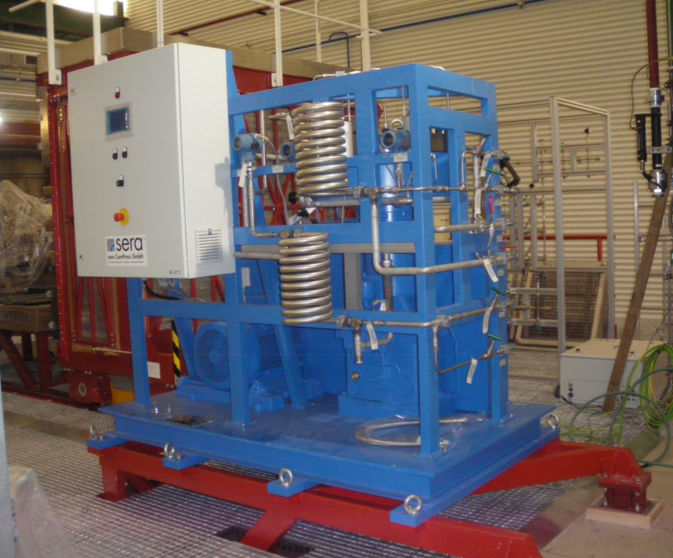
\includegraphics[width=\textwidth, ]{F13.png}}
        \caption{\textit{The compressor during the installation phase. The pedestal is shown in red. The control box, in white}}
        \label{fig:F13:F13}
    \end{center}
\end{figure}


\section{Safety procedures and risk assessment for NEW}
Several Process Procedures have been written to address specific operations in NEW commissioning and operation, describing hazards and defining safe working procedures. 
All of them have been approved by LSC.

Four new Process Procedures are being produced, to address the commissioning and operation of the field cage's high voltage, the use of radioactive sources and the 
commissioning and operation of the Gas systen in NEW. These Procedures will cover the range of (currently) intended operations.

\begin{figure}[ht!]
    \bigskip
    \begin{center}\leavevmode
        \rotatebox{0}{
        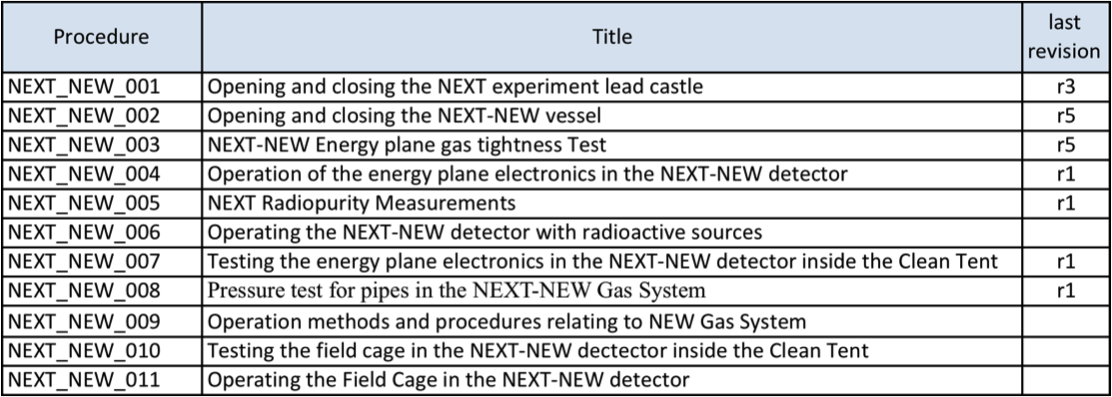
\includegraphics[width=\textwidth, ]{Procedures.png}}
        \caption{\textit{List of existing and in-preparation NEXT NEW Process Procedures}}
        \label{fig:PROC:PROC}
    \end{center}
\end{figure}


\subsection{Risk assessment for the Gas System}
A risk assessment review took place at LSC on 8th and 9th February 2016, organized by the LSC Director and counting with six experts from LNGS in the review panel.
The documentation (FMECA analysis, quantitative criticality analysis and a description of the gas system elements and operation, among other documents) as well as NEXT's working 
platform were reviewed.

Although no major problems were detected, a number of enhancements in the gas system design were suggested. 
Additionally, the panel advised to (1) carry out a HAZOP analysis leaded by an external company, (2) do gas flow calculations for the critical elements and 
(3) enhance the technical drawings for the gas system to adhere to the ISA Standard S5.1 Instrumentation Symbol Specification. 

A HAZOP analysis has been carried out with the help of the company Insegma (www.insegma.com) in March-April 2016. We are waiting to receive the final report, though we have already
used the analysis results to enhance the safety and reliability of the gas system.

The legalization of the Gas System is being prepared by an external company, Cryovac, who has carried out its own safety analysis and made requests and suggestions which have been already addressed.

Gas flow calculations have been carried out, validating the original design assumptions. The technical drawings are currently being updated to the ISA S5.1 standard.

Safety reviews at LSC, the one carried out by Cryovac and the HAZOP analysis by Insegma have been extremely useful to identify weak points and produce a better design and documentation. NEXT-NEW Process Procedure (Operating
methods and procedures relating to NEW gas system), which is to be submitted to LSC between 18th and 22nd April 2016, is the reference document for the gas system description and operation.

\subsection{Next steps}
LSC poses the following conditions to grant permission to operate the gas system with Argon and commercial/depleted Xenon between 5 and 10 bar: 
\begin{itemize}
\item Perform pressure tests for rigid pipes in the Gas system. Tests have been already carried out early in April.
\item Hand in the HAZOP analysis report and updated risk assessment documentation (including Process Procedure NEXT-NEW-009). The docuementation needs to be approved by LSC. NEXT will hand in these documentation in the third week in April.
\item Legalize of the pressure system according to national and regional regulations. The company Cryovac is taking care of this and the process should have concluded the last week of April.
\end{itemize}

Starting in May 2016, we plan to run, test and debug the detector throughout the rest of 2016. Learned lessons will allow us target operation up to 15 bar with enriched Xenon after the correspondign new risk assessment and, if applicable, gas system upgrade.

Also in May-June 2016, we intend to hand in an upgraded risk assessment, which will include the technical drawings according to the ISA S5.1 standard and an extension of the HAZOP to include the pneumatic system. The pneumatic system consists of a pressure tank constantly filled by LSC's pressure air line and three regulators which deliver the right actuation pressure for the different pneumatic valves and other components. Though not considered critical (pressure in the tank is monitored as well as the state -open/closed- of the pneumatic valves, so potential failures are detected and NEW automatically brought to the safe state), we aim at a high reliable operation and so decided to include this sub-system in the HAZOP.

\begin{figure}[ht!]
    \bigskip
    \begin{center}\leavevmode
        \rotatebox{0}{
        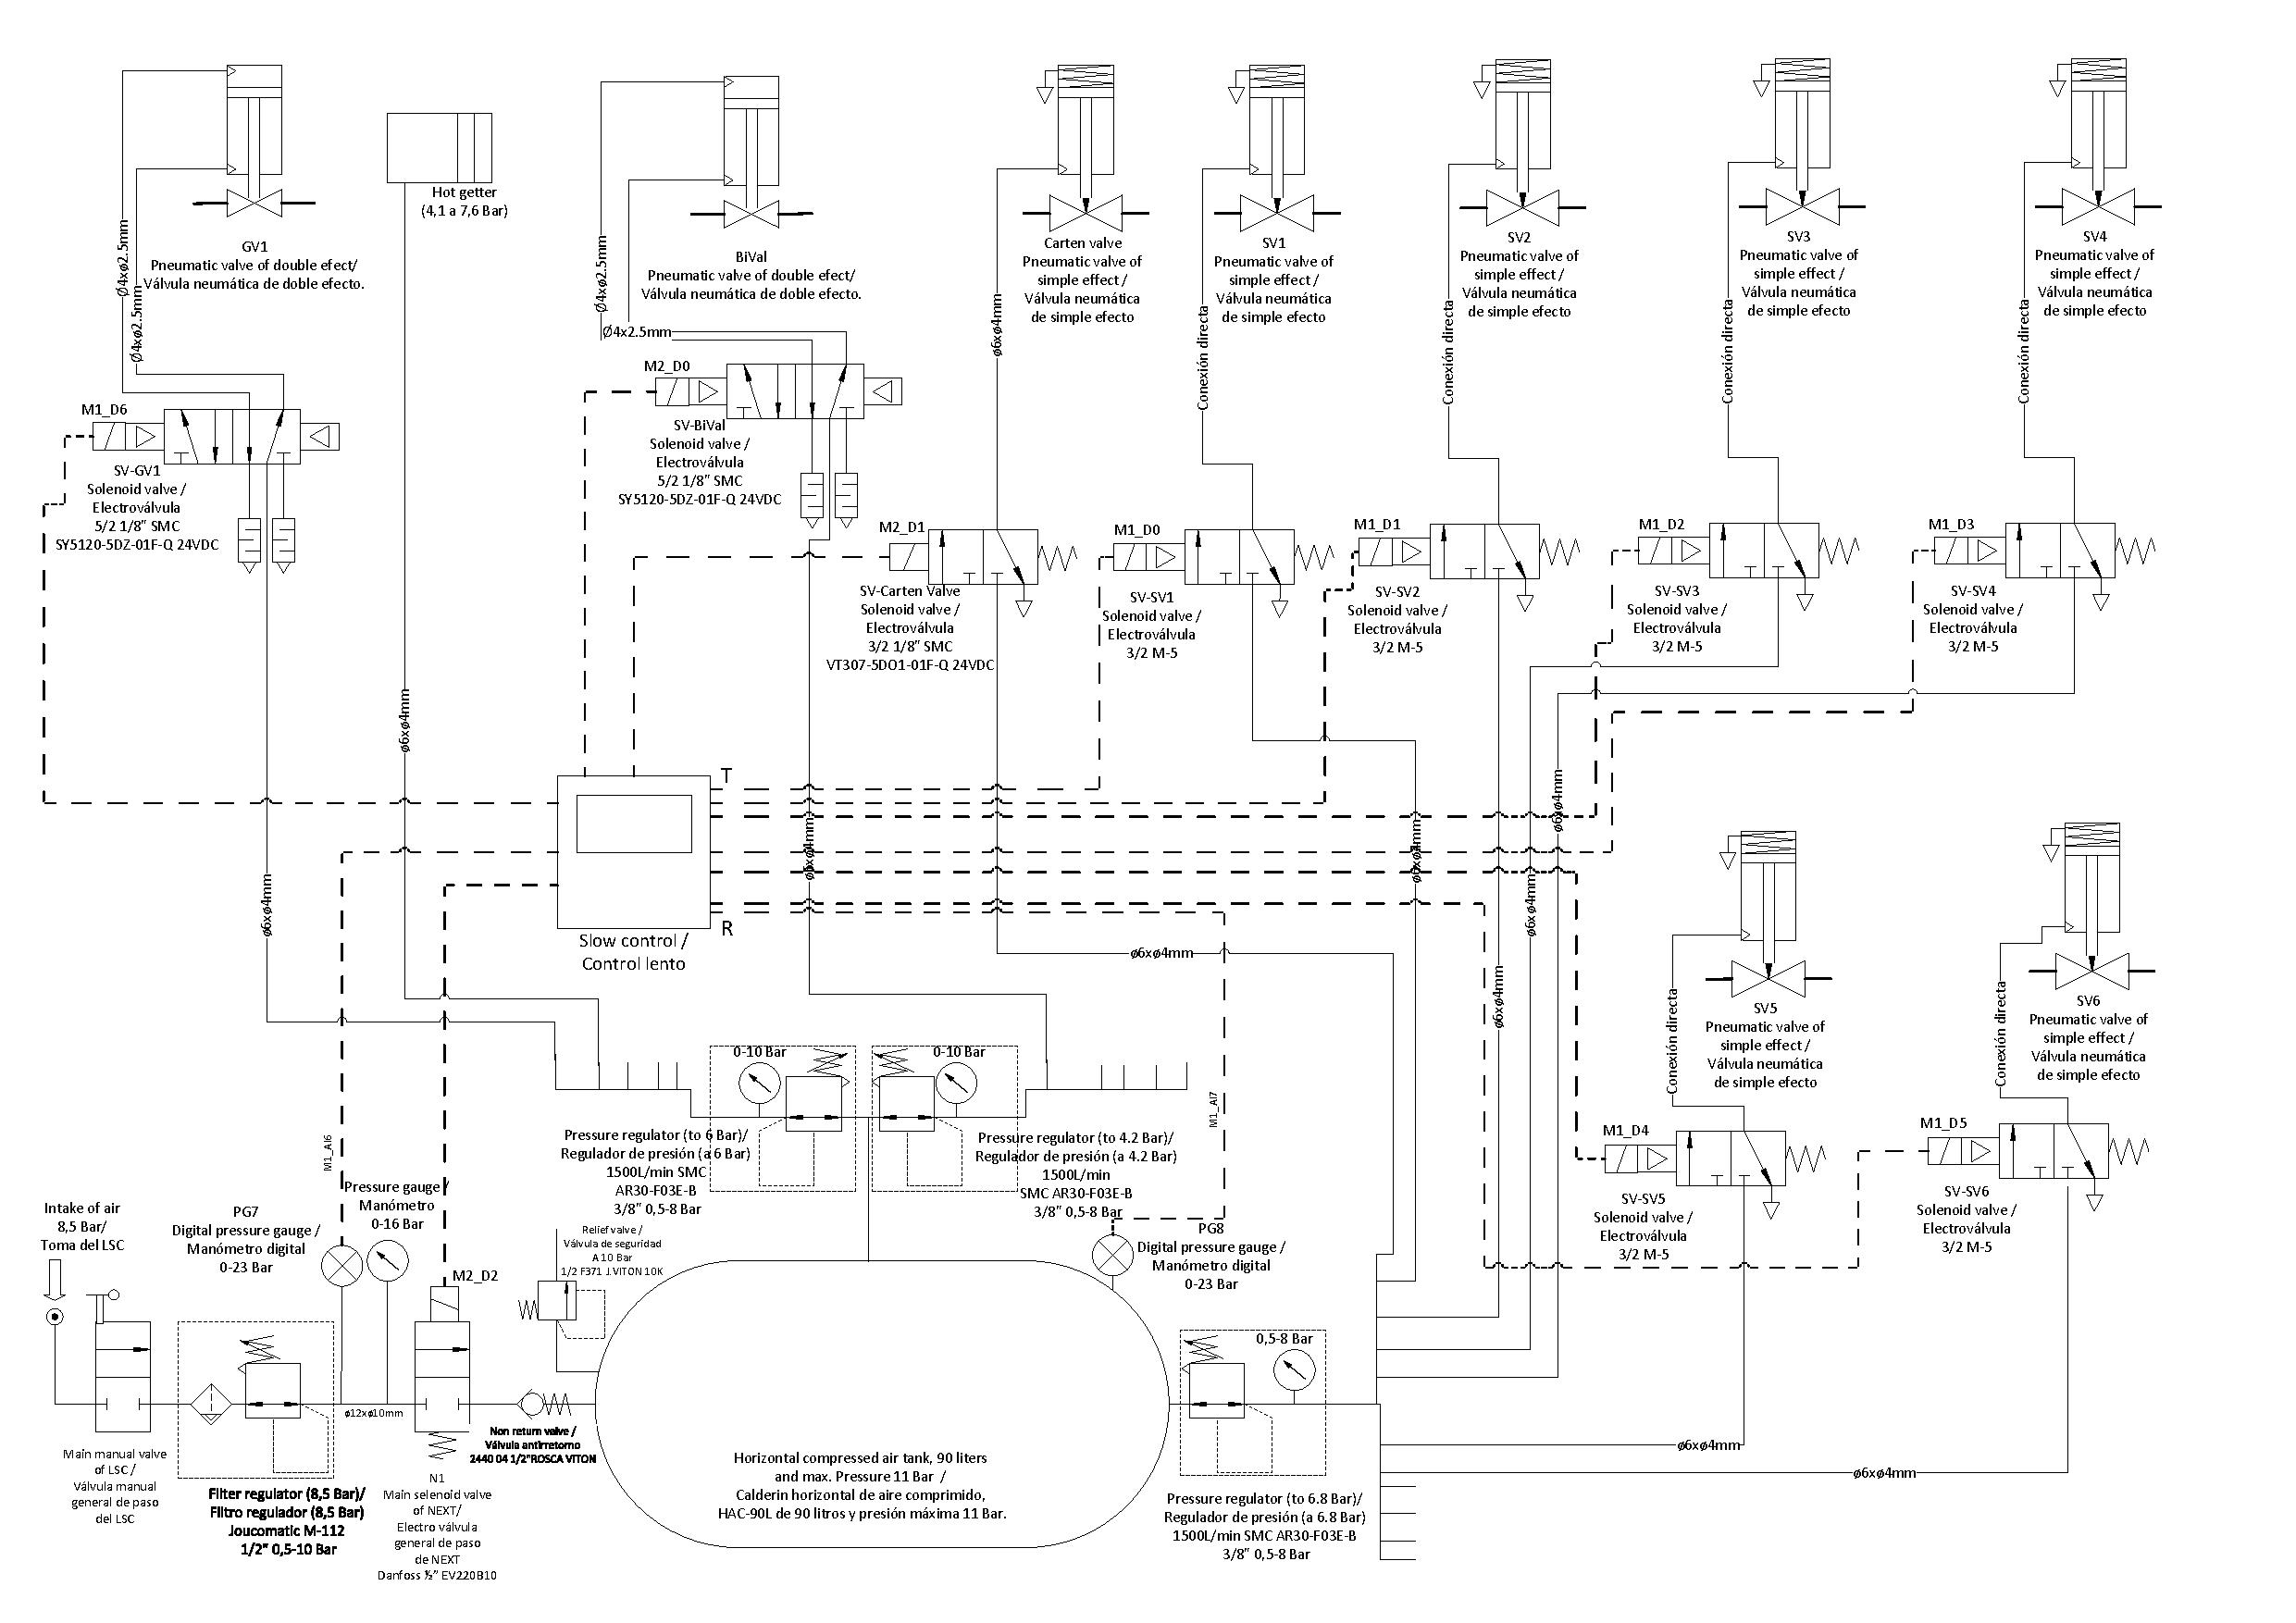
\includegraphics[width=\textwidth, ]{Pneumatic.pdf}}
        \caption{\textit{Pneumatic system scheme}}
        \label{fig:PNEU:PNEU}
    \end{center}
\end{figure}


\end{document}




